







\documentclass{article}\usepackage[]{graphicx}\usepackage[]{color}
%% maxwidth is the original width if it is less than linewidth
%% otherwise use linewidth (to make sure the graphics do not exceed the margin)
\makeatletter
\def\maxwidth{ %
  \ifdim\Gin@nat@width>\linewidth
    \linewidth
  \else
    \Gin@nat@width
  \fi
}
\makeatother

\definecolor{fgcolor}{rgb}{0.345, 0.345, 0.345}
\newcommand{\hlnum}[1]{\textcolor[rgb]{0.686,0.059,0.569}{#1}}%
\newcommand{\hlstr}[1]{\textcolor[rgb]{0.192,0.494,0.8}{#1}}%
\newcommand{\hlcom}[1]{\textcolor[rgb]{0.678,0.584,0.686}{\textit{#1}}}%
\newcommand{\hlopt}[1]{\textcolor[rgb]{0,0,0}{#1}}%
\newcommand{\hlstd}[1]{\textcolor[rgb]{0.345,0.345,0.345}{#1}}%
\newcommand{\hlkwa}[1]{\textcolor[rgb]{0.161,0.373,0.58}{\textbf{#1}}}%
\newcommand{\hlkwb}[1]{\textcolor[rgb]{0.69,0.353,0.396}{#1}}%
\newcommand{\hlkwc}[1]{\textcolor[rgb]{0.333,0.667,0.333}{#1}}%
\newcommand{\hlkwd}[1]{\textcolor[rgb]{0.737,0.353,0.396}{\textbf{#1}}}%

\usepackage{framed}
\makeatletter
\newenvironment{kframe}{%
 \def\at@end@of@kframe{}%
 \ifinner\ifhmode%
  \def\at@end@of@kframe{\end{minipage}}%
  \begin{minipage}{\columnwidth}%
 \fi\fi%
 \def\FrameCommand##1{\hskip\@totalleftmargin \hskip-\fboxsep
 \colorbox{shadecolor}{##1}\hskip-\fboxsep
     % There is no \\@totalrightmargin, so:
     \hskip-\linewidth \hskip-\@totalleftmargin \hskip\columnwidth}%
 \MakeFramed {\advance\hsize-\width
   \@totalleftmargin\z@ \linewidth\hsize
   \@setminipage}}%
 {\par\unskip\endMakeFramed%
 \at@end@of@kframe}
\makeatother

\definecolor{shadecolor}{rgb}{.97, .97, .97}
\definecolor{messagecolor}{rgb}{0, 0, 0}
\definecolor{warningcolor}{rgb}{1, 0, 1}
\definecolor{errorcolor}{rgb}{1, 0, 0}
\newenvironment{knitrout}{}{} % an empty environment to be redefined in TeX

\usepackage{alltt}
\IfFileExists{upquote.sty}{\usepackage{upquote}}{}
\begin{document}
\title{Overview of 
``divusa'' 
Dataset from 
``faraway''
Package}
\author{Julian Hatwell}
\maketitle

This document provides a brief overview of the
divusa dataset in the 
faraway R package.

\begin{knitrout}
\definecolor{shadecolor}{rgb}{0.969, 0.969, 0.969}\color{fgcolor}\begin{kframe}
\begin{verbatim}
##       year         divorce        unemployed         femlab     
##  Min.   :1920   Min.   : 6.10   Min.   : 1.200   Min.   :22.70  
##  1st Qu.:1939   1st Qu.: 8.70   1st Qu.: 4.200   1st Qu.:27.47  
##  Median :1958   Median :10.60   Median : 5.600   Median :37.10  
##  Mean   :1958   Mean   :13.27   Mean   : 7.173   Mean   :38.58  
##  3rd Qu.:1977   3rd Qu.:20.30   3rd Qu.: 7.500   3rd Qu.:47.80  
##  Max.   :1996   Max.   :22.80   Max.   :24.900   Max.   :59.30  
##     marriage          birth           military     
##  Min.   : 49.70   Min.   : 65.30   Min.   : 1.940  
##  1st Qu.: 61.90   1st Qu.: 68.90   1st Qu.: 3.469  
##  Median : 74.10   Median : 85.90   Median : 9.102  
##  Mean   : 72.97   Mean   : 88.89   Mean   :12.365  
##  3rd Qu.: 80.00   3rd Qu.:107.30   3rd Qu.:14.266  
##  Max.   :118.10   Max.   :122.90   Max.   :86.641
\end{verbatim}
\end{kframe}
\end{knitrout}

From the summary, and the associated help (not shown), the following observations can be made:
\newline

The dataframe contains 
77 
rows and 
7
columns. 

\newpage





\begin{knitrout}
\definecolor{shadecolor}{rgb}{0.969, 0.969, 0.969}\color{fgcolor}\begin{figure}
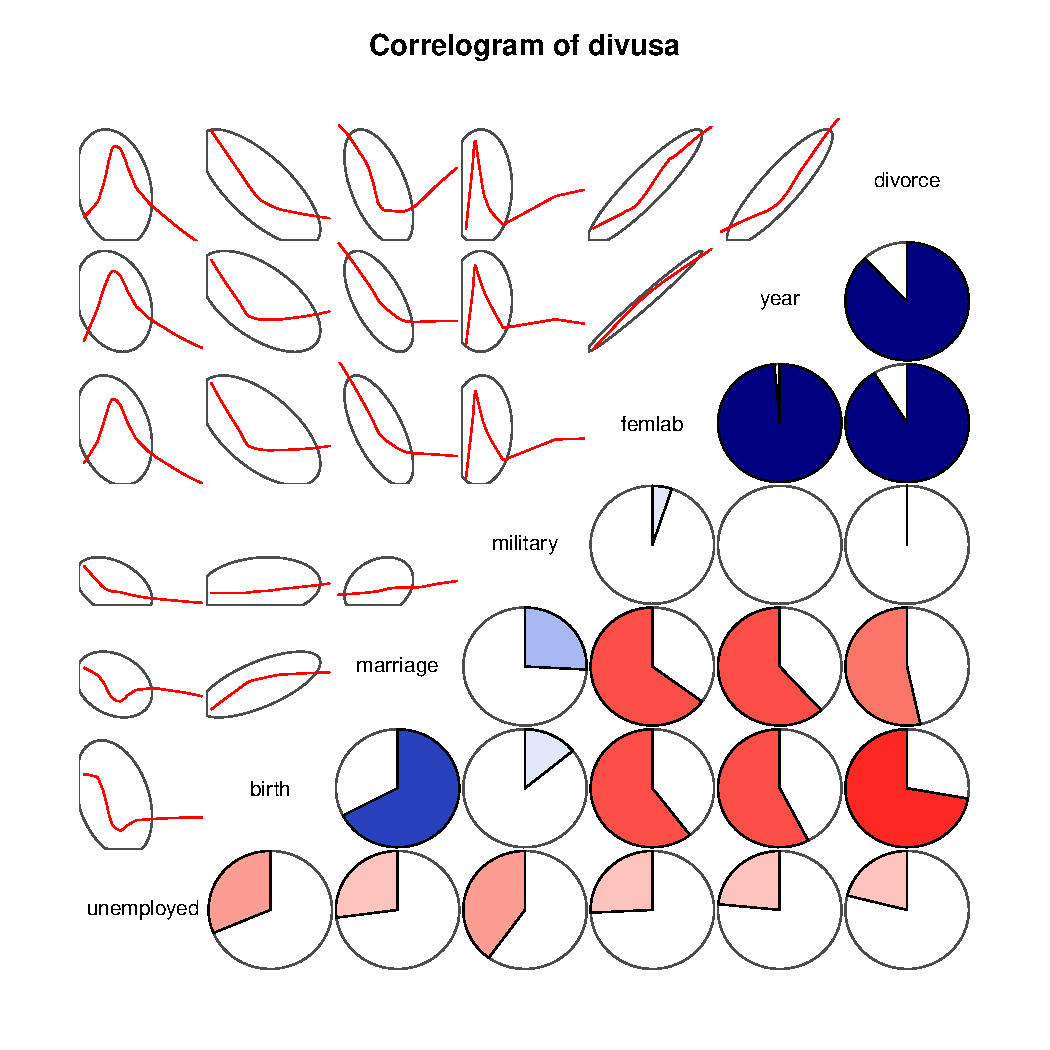
\includegraphics[width=\maxwidth]{figure/corrgram_custom-1} \caption[multi-variate comparisons]{multi-variate comparisons}\label{fig:corrgram_custom}
\end{figure}


\end{knitrout}





\begin{knitrout}
\definecolor{shadecolor}{rgb}{0.969, 0.969, 0.969}\color{fgcolor}\begin{figure}
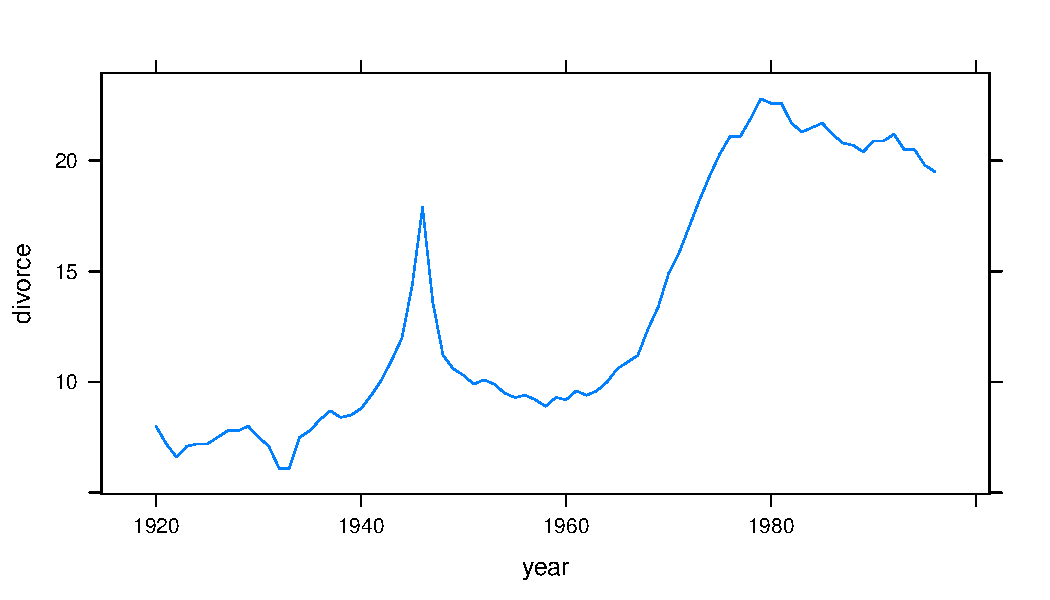
\includegraphics[width=\maxwidth]{figure/time_series-1} \caption[Time Series  plot of divorce against year]{Time Series  plot of divorce against year}\label{fig:time_series}
\end{figure}


\end{knitrout}


\begin{knitrout}
\definecolor{shadecolor}{rgb}{0.969, 0.969, 0.969}\color{fgcolor}\begin{figure}
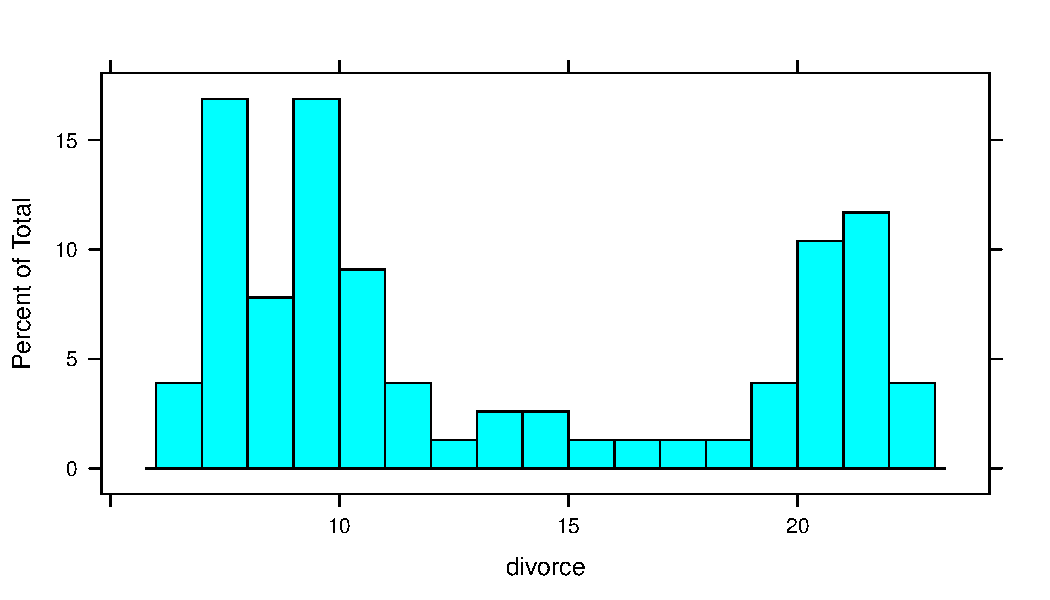
\includegraphics[width=\maxwidth]{figure/histograms-1} \caption[Histogram of the divorce variable]{Histogram of the divorce variable}\label{fig:histograms1}
\end{figure}

\begin{figure}
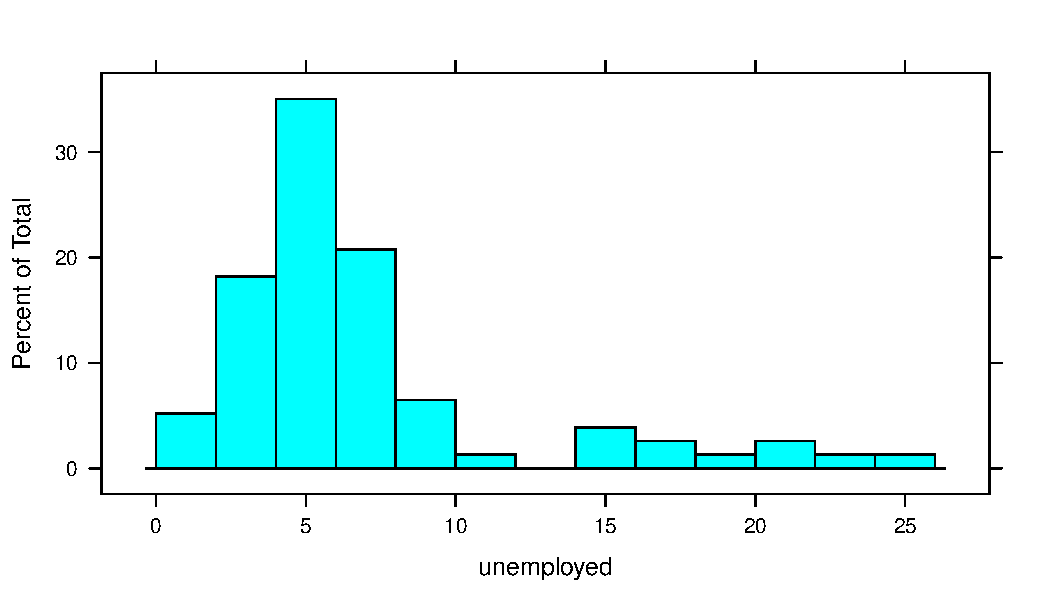
\includegraphics[width=\maxwidth]{figure/histograms-2} \caption[Histogram of the unemployed variable]{Histogram of the unemployed variable}\label{fig:histograms2}
\end{figure}

\begin{figure}
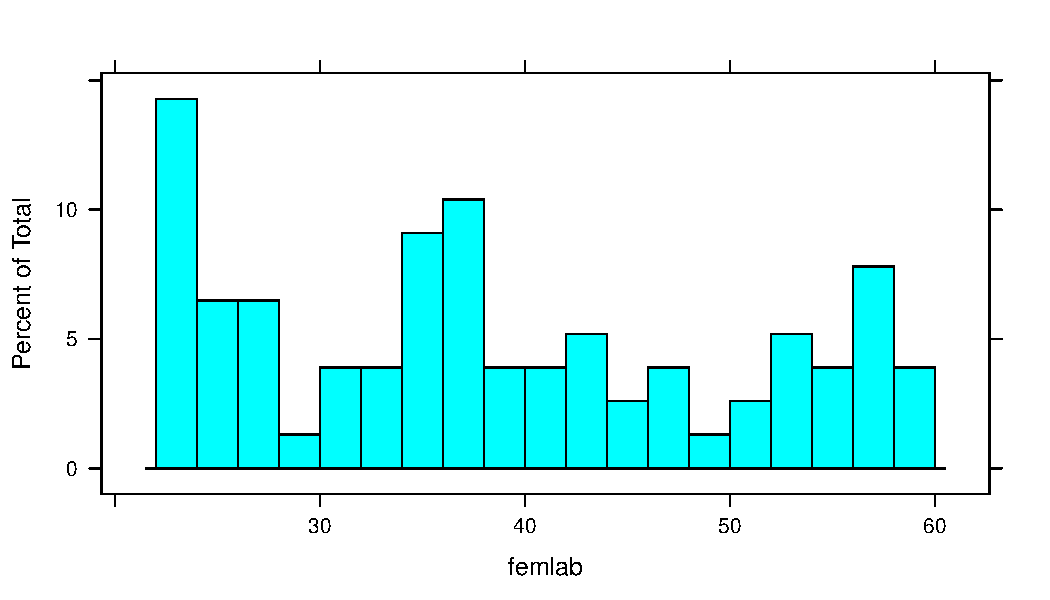
\includegraphics[width=\maxwidth]{figure/histograms-3} \caption[Histogram of the femlab variable]{Histogram of the femlab variable}\label{fig:histograms3}
\end{figure}

\begin{figure}
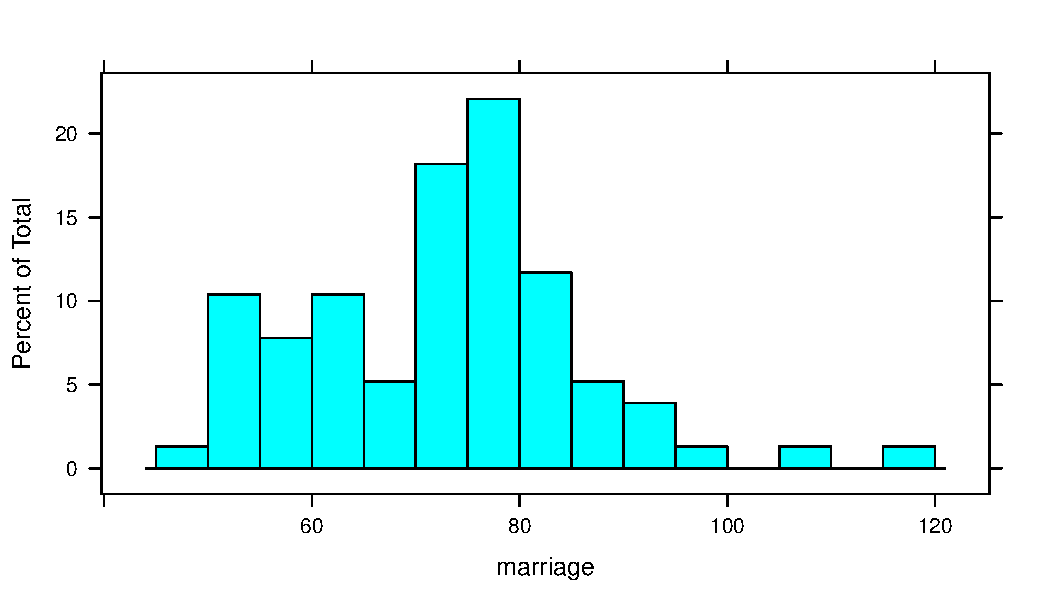
\includegraphics[width=\maxwidth]{figure/histograms-4} \caption[Histogram of the marriage variable]{Histogram of the marriage variable}\label{fig:histograms4}
\end{figure}

\begin{figure}
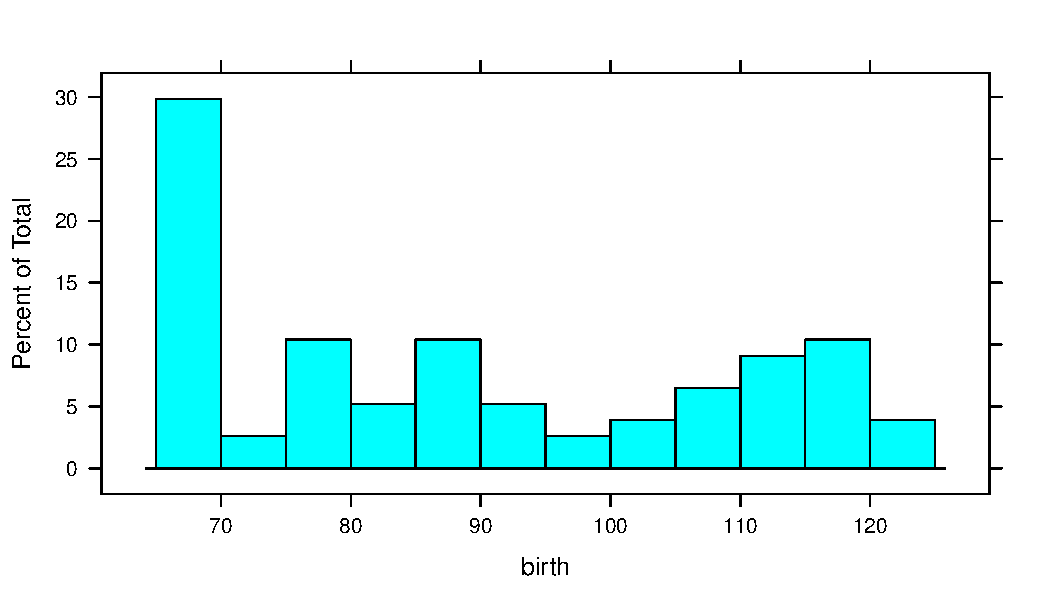
\includegraphics[width=\maxwidth]{figure/histograms-5} \caption[Histogram of the birth variable]{Histogram of the birth variable}\label{fig:histograms5}
\end{figure}

\begin{figure}
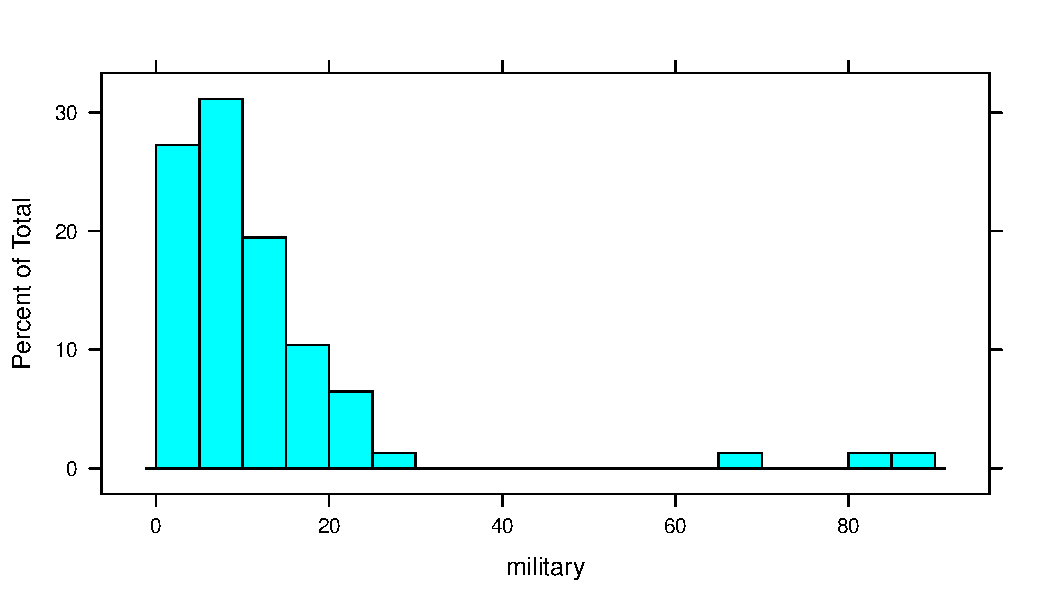
\includegraphics[width=\maxwidth]{figure/histograms-6} \caption[Histogram of the military variable]{Histogram of the military variable}\label{fig:histograms6}
\end{figure}


\end{knitrout}







\begin{knitrout}
\definecolor{shadecolor}{rgb}{0.969, 0.969, 0.969}\color{fgcolor}\begin{figure}
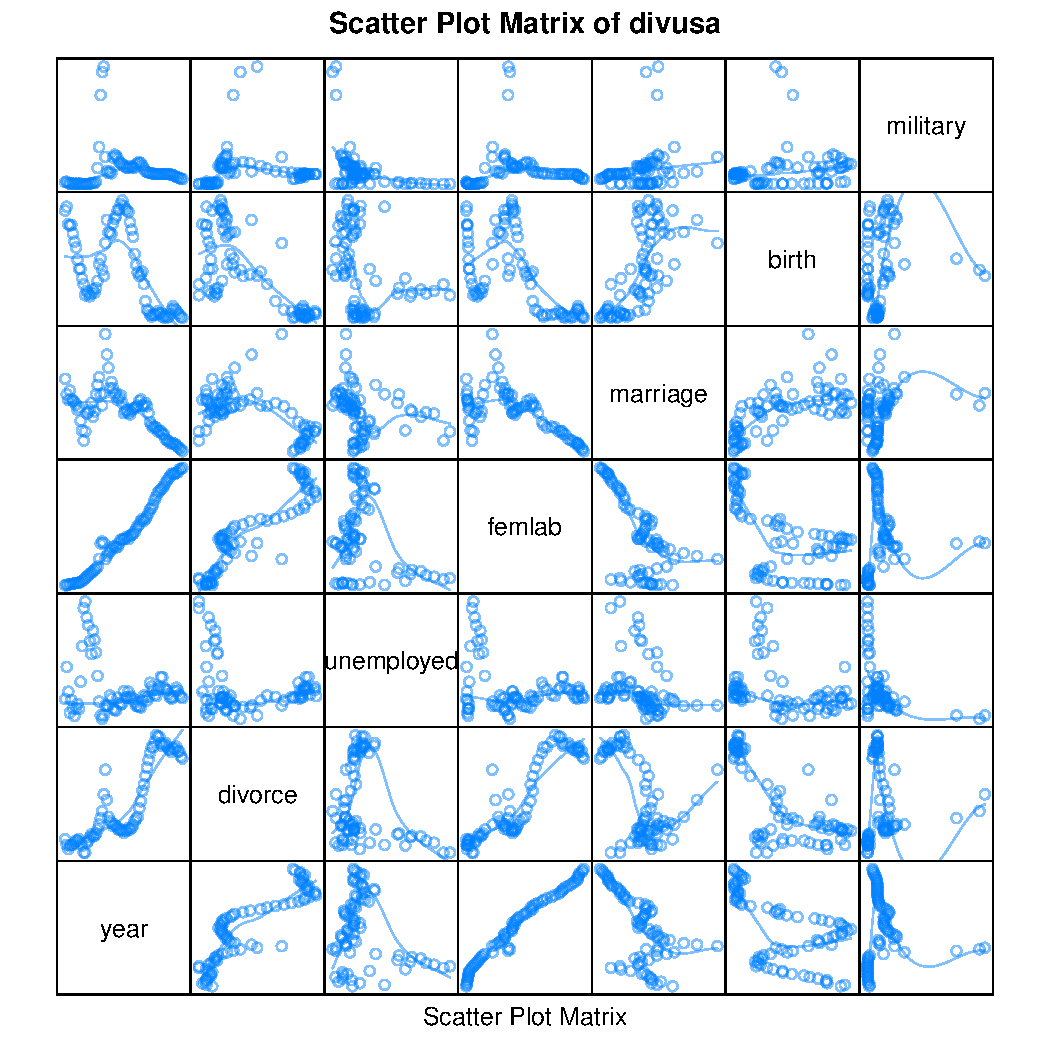
\includegraphics[width=\maxwidth]{figure/splom-1} \caption[multi-variate comparisons]{multi-variate comparisons}\label{fig:splom}
\end{figure}


\end{knitrout}






\begin{knitrout}
\definecolor{shadecolor}{rgb}{0.969, 0.969, 0.969}\color{fgcolor}\begin{kframe}
\begin{alltt}
\hlcom{# Year is an integer value and should be}
\hlcom{# used as a time series.}

\hlstd{df} \hlkwb{<-} \hlstd{df} \hlopt \hlkwd{mutate}\hlstd{(}\hlkwc{year} \hlstd{=} \hlkwd{ts}\hlstd{(year,} \hlkwc{frequency} \hlstd{=} \hlnum{1}\hlstd{))}
\end{alltt}
\end{kframe}
\end{knitrout}

\end{document}
